\documentclass{article}
\usepackage[spanish]{babel}
\usepackage{graphicx}
\usepackage{xcolor}
\usepackage[utf8]{inputenc}
\usepackage{fancyhdr}
\usepackage{lastpage}
\usepackage{enumitem}
\usepackage{listings}
\usepackage{verbatim}
\usepackage{float}

\pagestyle{fancy}
\fancyhf{}
\rfoot{Page \thepage\hspace{1pt} de~\pageref{LastPage}}

\title{}
\author{
Guillermo López García
\and
Guillermo Girón García
\and
Teodoro Martínez Márquez
}

\begin{document}
\maketitle

\textbf{1º Parte. Crear un repositorio en GitHub.}\\
\begin{figure}[H]
\centering
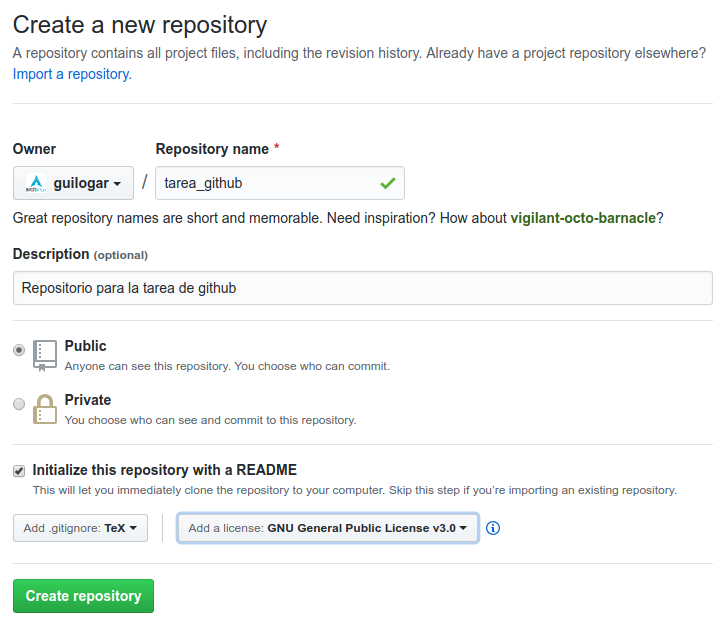
\includegraphics[width=0.7\linewidth]{./1_1}
\caption{Repositorio tarea\_github}
\end{figure}

\textbf{2º Parte. Realizar operaciones en el repositorio por todos los miembros (crear ficheros, modificarlos, borrarlos, etc\ldots) o tareas más avanzadas si se desea (por ejemplo, usar distintas ramas)}\\

\begin{figure}[H]
\centering
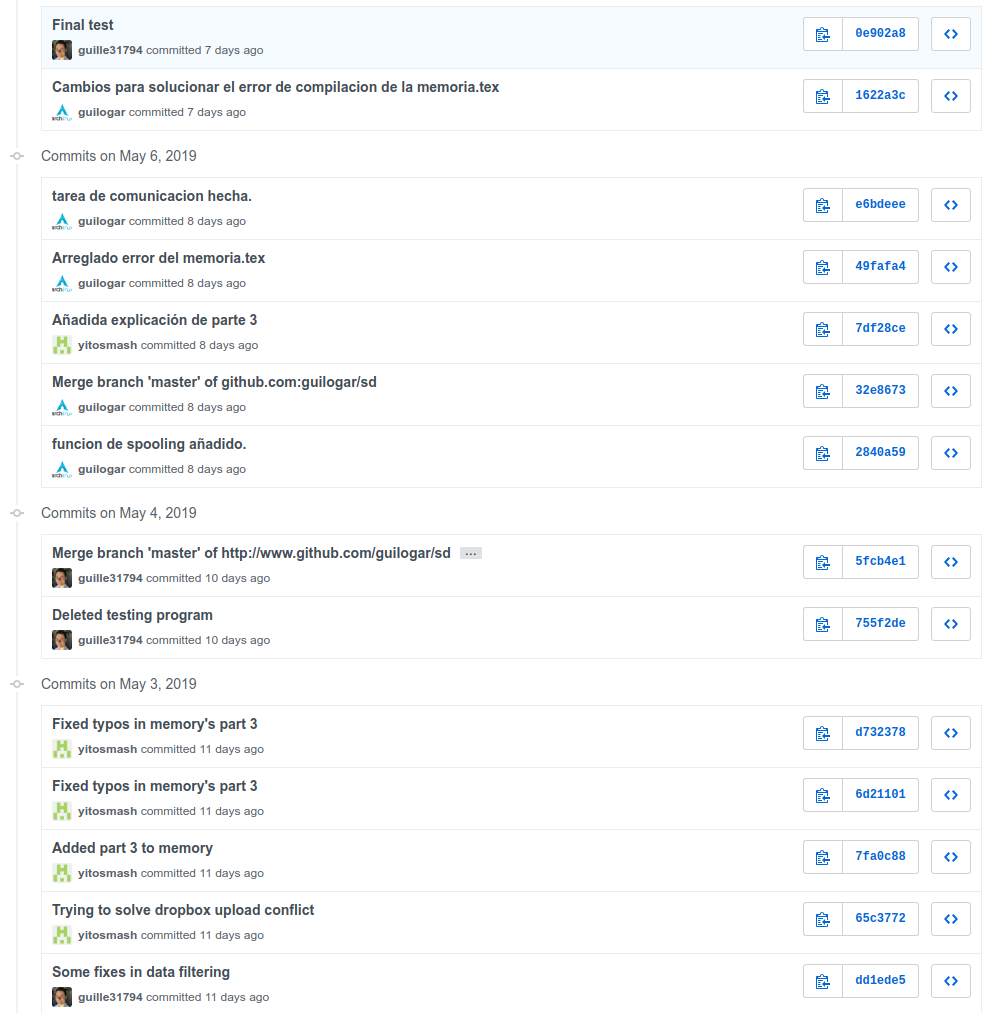
\includegraphics[width=0.7\linewidth]{./2_1}
\caption{Commits de los distintos componentes en el repositorio sd}
\end{figure}

\begin{figure}[H]
\centering
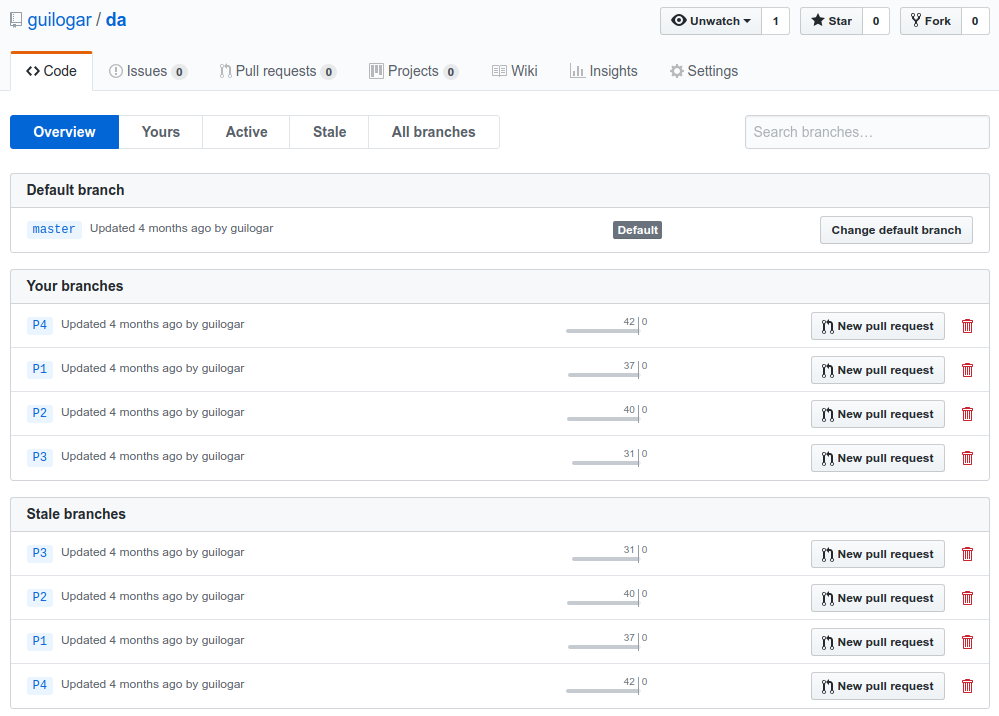
\includegraphics[width=0.7\linewidth]{./2_2}
\caption{Ramas en el repositorio da}
\end{figure}

\textbf{3º Parte. Probar algunas de las funcionalidades que ofrece Github (issues, pull requests\ldots)}\\

\begin{figure}[H]
\centering
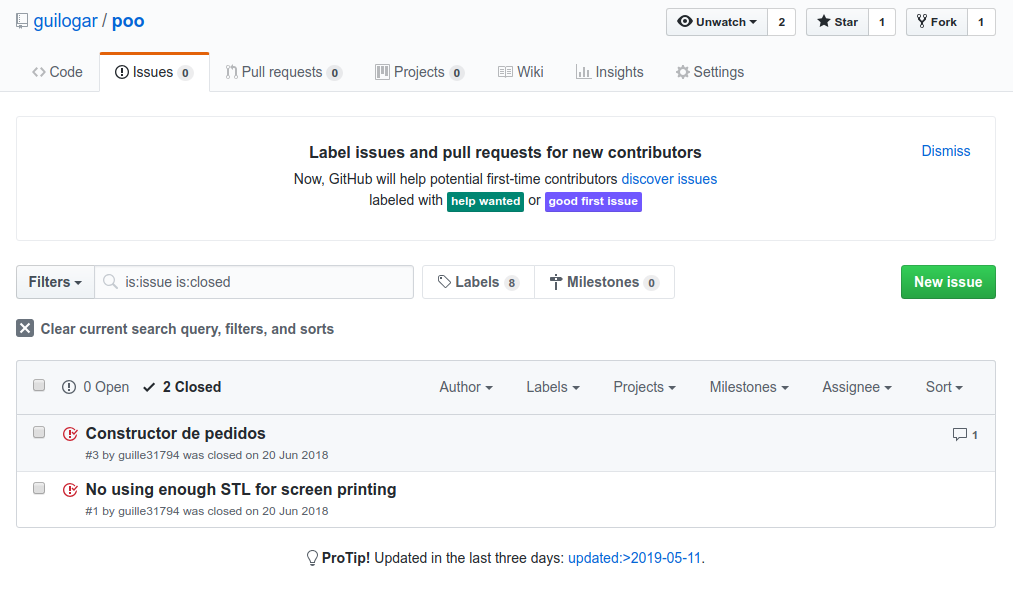
\includegraphics[width=0.7\linewidth]{./3_1}
\caption{Issues en el repositorio poo}
\end{figure}

\begin{figure}[H]
\centering
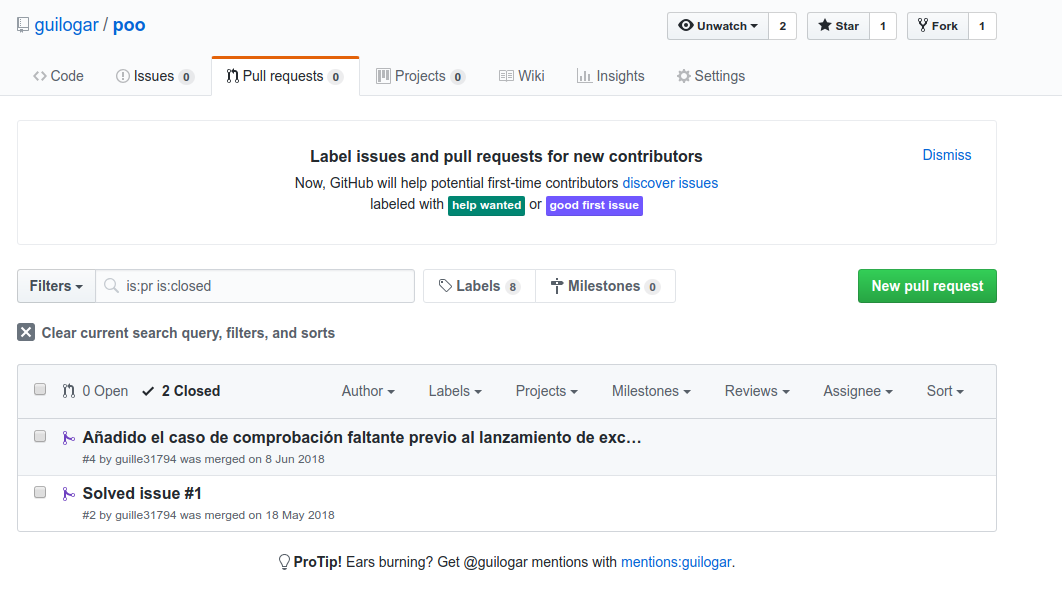
\includegraphics[width=0.7\linewidth]{./3_2}
\caption{Pull Request en el repositorio poo}
\end{figure}

%\begin{enumerate}%[label=\alph*]
    %\item \underline{}:
%\end{enumerate}
%\begin{itemize}
    %\item \underline{}:
%\end{itemize}
%\lstset{
  %language=...,
  %texcl=true,
  %basicstyle=\ttfamily,
  %columns=fullflexible,
  %frame=single,
  %breaklines=true,
  %postbreak=\mbox{\textcolor{red}{$\hookrightarrow$}\space},
%}
%\lstinputlisting[]{base_de_datos/sql.sql}
%\begin{figure}[H]
%\centering
%\includegraphics[width=0.7\linewidth]{./...}
%\caption{...}
%\end{figure}

\end{document}
